\documentclass{standalone}
\usepackage{tikz}
\usepackage{pgf-umlcd}
\usepackage{fontspec,xcolor,ifthen,xifthen}

\setmonofont[
    AutoFakeSlant,
    BoldItalicFeatures={FakeSlant},
]{Inconsolatazi4}

\newcommand{\fieldType}[2]{\texttt{\color{red}{#1:\hspace{1mm}#2}}}
\newcommand{\funcType}[4][]{\texttt{\color{blue}{#2(#3)%
    \ifthenelse{\isempty{#4}}%
    {}%
    {\hspace{1mm}#4}%
    \ifthenelse{\isempty{#1}}%
    {}%
    {:\hspace{1mm}#1}%
}}}

\begin{document}

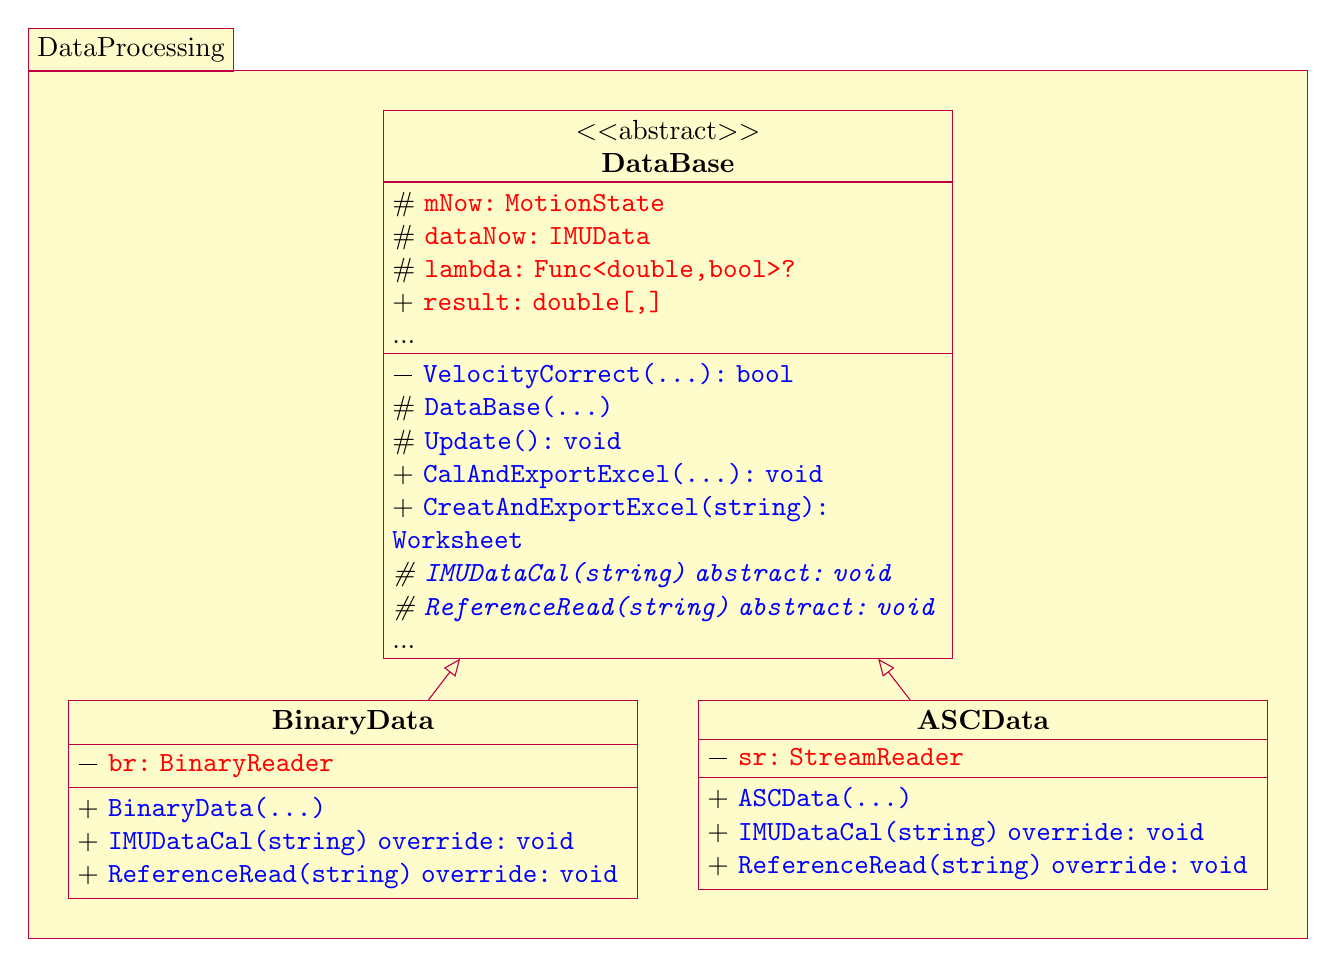
\begin{tikzpicture}
\begin{package}{DataProcessing}
\begin{abstractclass}[text width =7 cm]{DataBase}{0 ,1}
\attribute{\# \fieldType{mNow}{MotionState}}
\attribute{\# \fieldType{dataNow}{IMUData}}
\attribute{\# \fieldType{lambda}{Func<double,bool>?}}
\attribute{+ \fieldType{result}{double[,]}}
\attribute{...}
\operation{\textminus\phantom{ }\funcType[bool]{VelocityCorrect}{...}{}}
\operation{\# \funcType{DataBase}{...}{}}
\operation{\# \funcType[void]{Update}{}{}}
\operation{+ \funcType[void]{CalAndExportExcel}{...}{}}
\operation{+ \funcType[Worksheet]{CreatAndExportExcel}{string}{}}
\operation[0]{\# \funcType[void]{IMUDataCal}{string}{abstract}}
\operation[0]{\# \funcType[void]{ReferenceRead}{string}{abstract}}
\operation{...}
\end{abstractclass}
\begin{class}[text width =7cm]{BinaryData}{-4 , -6.5}
\inherit{DataBase}
\attribute{\textminus\phantom{ }\fieldType{br}{BinaryReader}}
\operation{+ \funcType{BinaryData}{...}{}}
\operation{+ \funcType[void]{IMUDataCal}{string}{override}}
\operation{+ \funcType[void]{ReferenceRead}{string}{override}}
\end{class}
\begin{class}[text width =7cm]{ASCData}{4 , -6.5}
\inherit{DataBase}
\attribute{\textminus\phantom{ }\fieldType{sr}{StreamReader}}
\operation{+ \funcType{ASCData}{...}{}}
\operation{+ \funcType[void]{IMUDataCal}{string}{override}}
\operation{+ \funcType[void]{ReferenceRead}{string}{override}}
\end{class}
\end{package}
\end{tikzpicture}

\end{document}